For the estimation of the rigid concepts the \acrfull{tps} mass and the structural mass estimates are combined to yield a single decelerator system mass value. This estimation is based on reference missions rather than structural models as employed for the mass estimates of the inflatable concepts. Steinfeldt \cite{Steinfeldt2009} provides one such mass estimate for a high mass Mars entry concept. Two concept are considered: a blunt body and a slender body of which the former is our primary interest. The reference missions used in Steinfeldts analysis are all of the blunt body type, similar to the rigid concept considered in this report. As such it is considered a very relative mass estimate method. The estimation provided below are all meant for such a blunt body.

Some remarks must however be made with regards to the use of these reference missions. Although rigid re-entry missions are plenty their relevance must be considered. Within this report a re-entry within the Martian atmosphere with a approach velocity of 7 [$km/s$] is considered. Most relevant reference missions are however for a planet different from Mars featuring a different re-entry trajectory. For the re-entry vehicles entering the Martian atmosphere the approach velocity may still be of a completely different order. Previously executed Martian entries were typically unmanned, featuring a Hohmann transfers to Mars in order to minimize propellent use. The mission at hand however features a more direct transfer considering human constraints yielding different approach velocities. As such the mass estimation should incorporate in some extend the thermal and structural loading of the mission trajectory.

The estimation provided by Steinfeldt takes this into account, dividing the estimation into three different parts: The forebody thermal protection system mass, the forebody structural mass and the back shell structural and thermal protection system mass estimate. The estimation takes into account the size of the concept by using the vehicles total mass at the start of the re-entry (\gls{sym:m0}). The heat load is taken into account by using the heat load \gls{sym:Q} and the structural loading is taken into account by using the peak dynamic pressure (\gls{sym:q}).

The mass estimate for the forebody thermal protection system is based in the heatload \gls{sym:Q} and is provided based on empirical analysis by \cite{Laub2004} in equation \ref{eq:tps_heat}\cite{Steinfeldt2009}:

\begin{equation}
\gls{sym:mheat} = (0.000091Q^{0.51575})\gls{sym:m0}
\label{eq:tps_heat}
\end{equation}

The mass estimate for the forebody structure is similarly given by equation \ref{eq:m_structure}\cite{Steinfeldt2009} depending the peak dynamic pressure:

\begin{equation}
\gls{sym:mstrcuture} = (0.0232 \gls{sym:q} ^{-0.1708} ) \gls{sym:m0}
\label{eq:m_structure}
\end{equation}

Applying the empirical relations with the design entry mass of $\gls{sym:m0} = 10000$ [$kg$] yield the relations as shown in figure \ref{fig:rigid}.

\begin{figure}[h]
	\centering
	\begin{subfigure}[b]{0.49\textwidth}
	\centering
	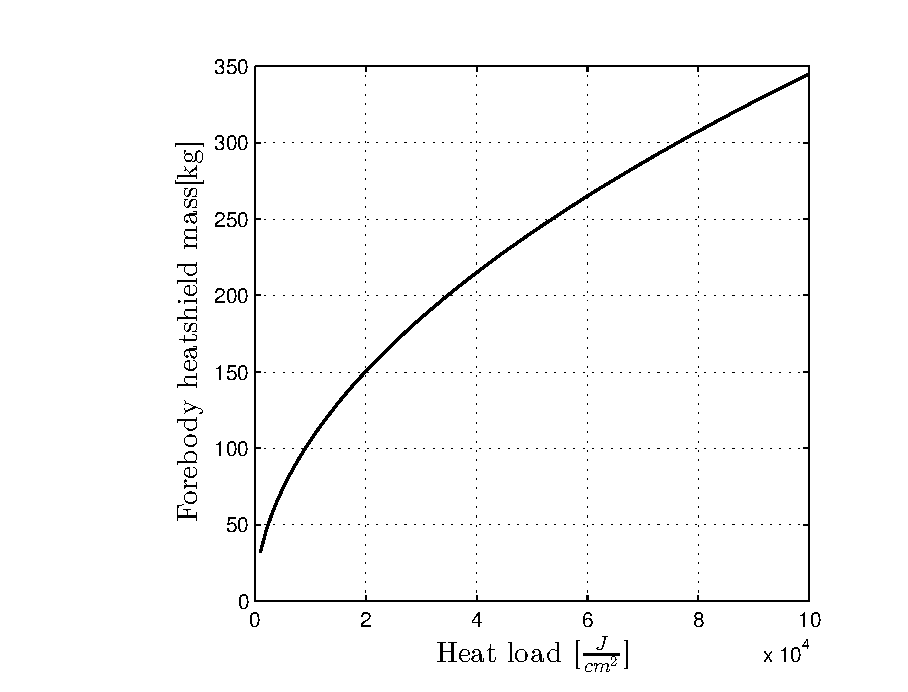
\includegraphics[width=1.0\textwidth]{Figure/rigidheat.eps}
	\caption{Empirical relation for the forebody heat shield mass} 
	\label{rigidheat}
	\end{subfigure}
	\begin{subfigure}[b]{0.49\textwidth}
	\centering
	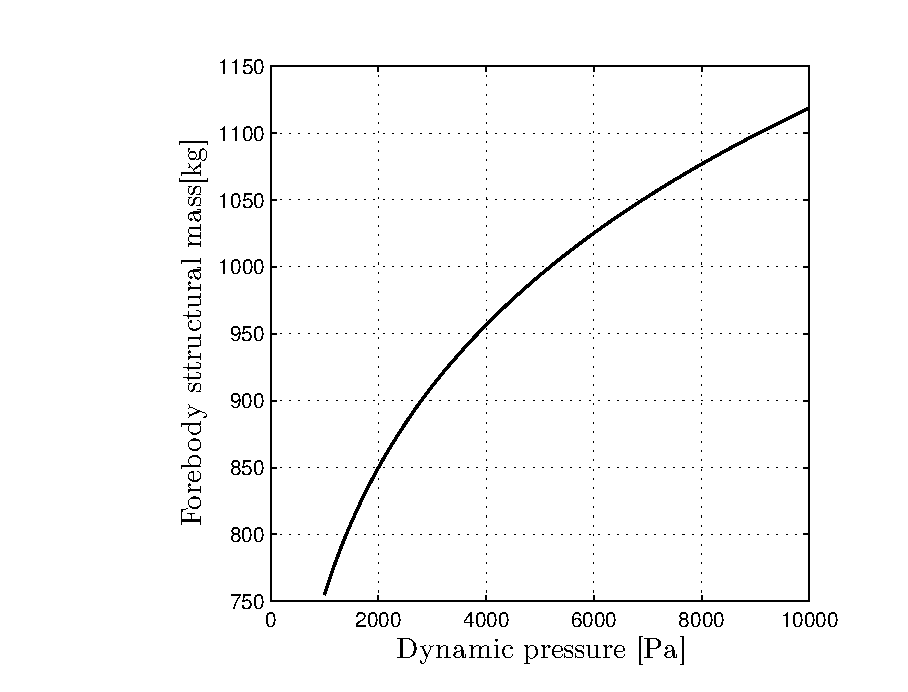
\includegraphics[width=1.0\textwidth]{Figure/rigidstruct.eps}
	\caption{Empirical relation for the forebody structural mass} 
	\label{fig:rigidstruct}
	\end{subfigure}
	\caption{Empirical relations for the forebody mass of a (blunt) rigid concept}
	\label{fig:rigid}
\end{figure}


Fig.\ref{fig:rigid} provides some sensitivity of the mass estimates with regard to trajectory. This allows for a first order estimate of the mass the rigid concept.

Moreover, different from the inflatable concepts a rigid design features a additional back shell structure \cite{Hughes:2005}. This backshell is required since the thermal loads cover also the backside of the structure. Streinfeldt suggest a value of 14\% of the total re-entry vehicle mass for the whole backshell thermal protection system and backshell structure. This would yield a backshell mass of $1400$ [kg] for the rigid concept at hand. The 14\% value should however be considered with care as their is no dependence on the thermal loads and structural loads in any form. Moroever it should be noted that part of this backshell structure may reduce the mass of the structural mass of the payload module.

Even tough the empirical relations stated above should be considered with strict care a crucial conclusion about the rigid concept can be made. Considering the best case scenario, with optimal loads and a large upwards bias of the empirical model the rigid concept will not be able to fulfil requirement ..??.. limiting the total decelerator mass to just $1000$ [$kg$]. Combining the above stated relations for the forebody heatshield mass, forebody structural mass and the backshell mass yields a value (way) above the $1000$ [$kg$] requirement.

Moreover the $1000$ [$kg$] mass requirement is for the whole decelerator concept. This also includes a control system which is not included within this mass estimate further reducing the viability of the rigid concept. 


This result is in line with Ref. \cite{Cianciolo2010} and \cite{Cassapakis1995} in which inflatable structures are already considered to be lighter than rigid structures.


Since the rigid concept will not be able to fulfil the set mission requirements the mass analysis for the rigid concept will not be detailed further. 

 


